\section{Kosten- und Nutzenanalyse}

In diesem Kapitel wird eine theoretische Kosten- und Nutzenanalyse der entwickelten Anwendung durchgeführt. Da die App zum Zeitpunkt dieser Arbeit noch nicht veröffentlicht wurde, basiert die Betrachtung ausschließlich auf geschätzten, potenziellen Einnahmen und Ausgaben. Ziel ist es, aufzuzeigen, welche wirtschaftlichen Möglichkeiten sich bei einem späteren Launch ergeben könnten und welches Einnahmepotenzial grundsätzlich vorhanden ist.

Die Analyse konzentriert sich daher auf mögliche Monetarisierungsmodelle, erwartbare Nutzerzahlen sowie daraus ableitbare Einnahmen, beispielsweise durch Werbung, In-App-Käufe oder andere Geschäftsmodelle. Den potenziellen Einnahmen werden geschätzte laufende Betriebskosten wie Serverkosten oder Infrastruktur gegenübergestellt.

Die während der Entwicklung angefallenen beziehungsweise anfallenden Entwicklungskosten werden in dieser Analyse bewusst nicht berücksichtigt, da der Fokus ausschließlich auf der theoretischen Wirtschaftlichkeit im laufenden Betrieb der Anwendung liegt.
\section{Skalierungsstrategie}

Um eine bestehende App-Infrastruktur an stark wachsende Nutzerzahlen anzupassen, müssen konkrete technologische Entscheidungen getroffen werden. Dabei stellt sich nicht nur die Frage \emph{wie} skaliert wird (vertikal oder horizontal), sondern insbesondere \emph{mit welchen Diensten und Infrastrukturmodellen} die Skalierung technisch umgesetzt werden soll. Im Folgenden werden zentrale Cloud- und Backend-Ansätze gegenübergestellt und hinsichtlich ihrer Eignung für kurzfristiges sowie langfristiges Nutzerwachstum bewertet.

\subsection{On-Premise vs. Cloud-Infrastruktur}

Eine klassische On-Premise-Architektur bietet volle Kontrolle über Hardware und Daten, ist jedoch bei starkem Wachstum unflexibel. Neue Server müssen physisch beschafft, installiert und konfiguriert werden. Dies verursacht hohe Vorlaufzeiten und Investitionskosten.

Cloud-Infrastrukturen (z.\,B. AWS, Google Cloud, Microsoft Azure) ermöglichen dagegen die dynamische Bereitstellung von Ressourcen. Virtuelle Maschinen oder Container können innerhalb weniger Minuten gestartet werden. Für eine wachsende App ist die Cloud daher deutlich besser geeignet, da Skalierung nahezu in Echtzeit erfolgen kann.

\textbf{Bewertung:}  
Für eine App mit potenziell stark steigender Nutzerzahl ist eine Cloud-basierte Infrastruktur klar vorzuziehen, da sie flexible Skalierung ohne hohe Anfangsinvestitionen erlaubt.

\subsection{IaaS vs. PaaS vs. BaaS}

Bei der Auswahl des Cloud-Ansatzes existieren unterschiedliche Abstraktionsebenen:

\textbf{Infrastructure as a Service (IaaS):}  
Hier werden virtuelle Server bereitgestellt. Entwickler verwalten Betriebssystem, Runtime und Deployment selbst. Vorteil ist maximale Kontrolle. Nachteil ist hoher administrativer Aufwand. Skalierung erfolgt über zusätzliche Instanzen und Load Balancer.

\textbf{Platform as a Service (PaaS):}  
Der Anbieter übernimmt Betriebssystem und Laufzeitumgebung. Deployment erfolgt automatisiert (z.\,B. per Git-Push). Skalierung kann oft per Klick oder automatisch konfiguriert werden. Der Verwaltungsaufwand ist geringer als bei IaaS.

\textbf{Backend as a Service (BaaS):}  
Plattformen wie Supabase oder Firebase stellen Datenbank, Authentifizierung, Realtime-Funktionen und APIs direkt bereit. Skalierung wird größtenteils vom Anbieter übernommen. Entwickler konzentrieren sich auf die App-Logik.

\textbf{Vergleich:}

\begin{itemize}
\item IaaS: maximale Flexibilität, geeignet für komplexe Systeme mit hoher Individualisierung
\item PaaS: gute Balance zwischen Kontrolle und Automatisierung
\item BaaS: schnellste Skalierung mit minimalem Infrastrukturaufwand
\end{itemize}

\textbf{Empfehlung:}  
Für eine wachsende App in frühen bis mittleren Phasen ist BaaS oder PaaS besonders geeignet, da Skalierungsmechanismen bereits integriert sind. Bei sehr großen Systemen mit speziellen Anforderungen kann langfristig ein Wechsel zu IaaS sinnvoll sein.

\subsection{Serverbasierte Architektur vs. Serverless}

\textbf{Klassische serverbasierte Architektur:}  
Backend läuft auf dauerhaft aktiven Serverinstanzen. Skalierung erfolgt durch Hinzufügen weiterer Instanzen (Autoscaling). Vorteil ist konstante Performance und volle Kontrolle. Nachteil sind laufende Kosten auch bei geringer Nutzung.

\textbf{Serverless / Function-as-a-Service (FaaS):}  
Code wird ereignisgesteuert ausgeführt. Ressourcen werden automatisch skaliert. Es fallen nur Kosten bei tatsächlicher Nutzung an. Ideal bei stark schwankender Last.

\textbf{Vergleich:}

\begin{itemize}
\item Serverbasiert: stabil bei konstant hoher Last
\item Serverless: flexibel bei stark variabler Last
\end{itemize}

\textbf{Empfehlung:}  
Für Apps mit unvorhersehbarem Wachstum oder saisonalen Peaks ist Serverless besonders geeignet. Bei dauerhaft hoher Nutzerzahl kann eine hybride Lösung sinnvoll sein.

\subsection{Datenbankstrategien}

\textbf{Single-Instance-Datenbank:}  
Einfach, aber bei hoher Last schnell überfordert.

\textbf{Read-Replicas:}  
Leseanfragen werden auf mehrere Replikate verteilt. Geeignet bei hohem Leseaufkommen.

\textbf{Sharding:}  
Aufteilung großer Datenmengen auf mehrere Datenbankinstanzen. Geeignet bei extrem großen Nutzerzahlen.

\textbf{Relationale vs. NoSQL-Datenbanken:}  
Relationale Systeme bieten hohe Konsistenz. NoSQL-Systeme sind oft horizontal besser skalierbar.

\textbf{Empfehlung:}  
Bei moderatem Wachstum reichen Read-Replicas aus. Bei massivem Wachstum ist Sharding oder ein verteilter Datenbankansatz notwendig.

\subsection{Organisatorische Skalierungsstrategien}

Technische Infrastruktur allein genügt nicht. Organisatorisch sind folgende Maßnahmen notwendig:

\begin{itemize}
\item Einführung von Monitoring-Systemen zur Lastüberwachung
\item Regelmäßige Lasttests
\item Automatisierte Deployments (CI/CD)
\item Klare Trennung von Entwicklungs-, Test- und Produktionsumgebung
\item Skalierbare Teamstrukturen (z.\,B. Aufteilung in Backend-, Infrastruktur- und Feature-Teams)
\end{itemize}

\subsection*{\textbf{Gesamtbewertung für eine wachsende App}}

Für eine moderne mobile App mit potenziell stark steigender Nutzerzahl ist folgende Kombination besonders geeignet:

\begin{itemize}
\item Cloud-basierte Infrastruktur statt On-Premise
\item PaaS oder BaaS in frühen Phasen
\item Autoscaling + Load Balancing
\item Caching und Datenbank-Replikation
\item Kontinuierliches Monitoring und automatisierte Deployments
\end{itemize}

Zusammenfassend lässt sich feststellen, dass kurzfristige Skalierung vor allem durch Cloud-Ressourcen, Autoscaling und Replikation erreicht wird, während langfristige Stabilität durch architektonische Modularisierung, optimierte Datenbankstrategien und organisatorische Prozesse gewährleistet wird. Die optimale Lösung hängt dabei vom Entwicklungsstand, Budget und erwarteten Nutzerwachstum der jeweiligen App ab.

\section{Evaluierung geeigneter Monetarisierungsstrategien}
In diesem Kapitel werden die zuvor beschriebenen Monetarisierungsansätze hinsichtlich ihrer Eignung für die entwickelte App bewertet und daraus eine empfohlene Strategie abgeleitet. Die App verursacht laufende Betriebskosten (insbesondere durch die Nutzung der Google Street View API). Daraus ergibt sich als zentrale Anforderung, dass die Monetarisierung \textit{wiederkehrende} bzw. kontinuierlich skalierende Einnahmen ermöglichen muss, welche im Idealfall die Kosten decken.

\subsection{Bewertungskriterien}
Für die Evaluierung werden folgende Kriterien herangezogen:
\begin{itemize}
    \item \textbf{Planbarkeit der Einnahmen:} Eignung für laufende Kosten und langfristigen Betrieb.
    \item \textbf{Skalierbarkeit:} Steigen die Einnahmen mit der Nutzerzahl ohne proportionale Mehrkosten?
    \item \textbf{Nutzererlebnis (UX):} Einfluss auf Spielfluss, Interface und wahrgenommene Qualität.
    \item \textbf{Umsetzbarkeit:} Technische Komplexität und Realisierbarkeit im Rahmen des Projekts.
    \item \textbf{Akzeptanz:} Wahrscheinlichkeit, dass Nutzer das Modell annehmen (Werbung/Abos/IAP).
\end{itemize}

\subsection{Nicht priorisierte Modelle}
\textbf{Spenden \& Crowdfunding} werden für diese App nicht als primäre Monetarisierung berücksichtigt. Der Hauptgrund ist die fehlende Einnahmensicherheit: freiwillige Beiträge sind schwer prognostizierbar und eignen sich daher nur eingeschränkt zur Deckung laufender API-Kosten. Als ergänzendes Modell (z.\,B. Community-Support) wäre es zwar denkbar, wird jedoch nicht als tragende Säule empfohlen.

\textbf{Sponsoring \& Partnerschaften} (z.\,B. mit Hotelbetrieben oder Tourismus-Organisationen) könnten mittelfristig attraktiv sein, sind jedoch in der Startphase meist schwer umsetzbar. Ohne nachweisbare Reichweite (aktive Nutzer, Spielrunden, Retention) ist die Verhandlungsposition schwach und Sponsoren erwarten üblicherweise messbare \gls{KPIs}. Daher wird Sponsoring als \textit{spätere} Option eingeordnet, sobald eine ausreichende Nutzerbasis aufgebaut wurde.

\textbf{Einmaliger Kauf} (Paid App) wird als ungeeignet bewertet. Ein Einmalkauf erzeugt zwar sofortige Einnahmen, passt jedoch schlecht zu laufenden Betriebskosten, da nach dem Kauf keine wiederkehrenden Erlöse entstehen. Zudem stellt der Kaufpreis eine Einstiegshürde dar, insbesondere im Spielebereich, in dem kostenlose Alternativen dominieren.

\subsection{Empfohlene Strategie: Hybridmodell aus Werbung, Pro-Abo und In-App-Käufen}
Als am besten geeignet wird ein \textbf{Hybridmodell} bewertet, das drei Elemente kombiniert:
\begin{enumerate}
    \item \textbf{Video-/Playable-Werbung als Basiserlös (Free-Nutzer)}
    \item \textbf{Pro-Abonnement als wiederkehrende Einnahmequelle (No-Ads)}
    \item \textbf{In-App-Käufe für kosmetische Inhalte (z.\,B. Profilbilder)}
\end{enumerate}

Dieses Modell ist in Mobile Games verbreitet, da es sowohl eine breite kostenlose Nutzung ermöglicht als auch zahlungsbereite Nutzer gezielt monetarisiert, ohne alle Nutzer zu einem Kauf zu zwingen.

\subsubsection{Werbung (Fokus: Rewarded Video und Playable Ads)}
Da die App ein Spiel ist, bieten sich insbesondere \textbf{vollflächige Formate} (Rewarded Video / Playables) an. Diese erzielen typischerweise höhere \gls{eCPM}-Werte als Banner, sind aber stärker in den Spielfluss integriert zu planen, um Frustration zu vermeiden. Rewarded Video \gls{eCPM} wird in Marktübersichten häufig im Bereich von etwa \textbf{10--50 USD pro 1.000 Impressionen} genannt (stark abhängig von Land, Zielgruppe und Nachfrage). \cite{BoA_RewardedVideo}

\textbf{Werbenetzwerk:} Für die theoretische Umsetzung wird \textbf{Google AdMob} vorgesehen, da es als verbreitetes Werbenetzwerk einen standardisierten Einstieg ermöglicht und die genannten Formate unterstützt.

\paragraph{Geplante Werbeplatzierungen (theoretisches Konzept)}
\mbox{}\\
Um eine Balance aus Einnahmen und UX zu erreichen, werden Werbeeinblendungen bevorzugt an \textbf{natürlichen Unterbrechungen} platziert:
\begin{itemize}
    \item \textbf{Mehrspieler:} nach jeder abgeschlossenen Runde ein Video/Playable (da klarer Abschlussmoment).
    \item \textbf{Daily Challenge:} nach Abschluss der Challenge ein Video/Playable.
    \item \textbf{Einzelspieler:} nach jeweils 5 Runden ein Video/Playable.
    \item \textbf{Menü-Rückkehr:} optional beim freiwilligen Zurückgehen ins Hauptmenü (z.\,B. nach 3 Runden), da dies weniger störend wirkt als während aktiver Spielphasen.
\end{itemize}

Zusätzlich kann ein \textbf{Werbung-gegen-Spielzeit}-Mechanismus eingesetzt werden:
\begin{itemize}
    \item Free-Nutzer erhalten z.\,B. \textbf{5 Einzelspieler-Spiele pro Tag}.
    \item Weitere Spiele können durch das Ansehen eines Rewarded Videos „freigeschaltet“ werden.
\end{itemize}
Dieser Ansatz ist aus UX-Sicht oft akzeptabler als erzwungene Unterbrechungen, da Nutzer die Werbung \textit{aktiv} zur Freischaltung wählen.

\paragraph{Banner-Werbung (bewusst zurückhaltend)}
\mbox{}\\
Banner werden weiterhin als kritisch bewertet, da sie UI-Flächen belegen und bei zu auffälliger Gestaltung die wahrgenommene Qualität der App reduzieren können. In diesem Konzept wird daher ein \textbf{kleiner, unaufdringlicher Banner am unteren Bildschirmrand} eingesetzt, der \textbf{auf allen Seiten außerhalb des aktiven Spiels} sichtbar ist (z.\,B. Menü, Lobby oder Profil). Während einer laufenden Spielrunde wird bewusst \textbf{kein Banner eingeblendet}, um den Spielfluss nicht zu stören. Durch diese Platzierung bleibt die Werbung dauerhaft sichtbar, ohne zentrale Interaktionsflächen zu überdecken. Primär wird dennoch auf \textbf{Video- bzw. Playable-Ads} fokussiert, da diese in der Regel höhere Einnahmen pro Impression erzielen und gezielt an natürlichen Unterbrechungspunkten im Spiel eingesetzt werden können.
\subsubsection{Pro-Abonnement (No-Ads)}
Ein Pro-Abo wird als besonders geeignet bewertet, weil es \textbf{wiederkehrende Einnahmen} ermöglicht und damit laufende Kosten (API) langfristig besser abdecken kann. Der Mehrwert ist für Nutzer klar kommunizierbar: \textbf{werbefreies Spielen} (und optional weitere Komfortfunktionen).

Für die erwartete Abo-Quote kann man sich an typischen Conversion-Ranges orientieren. Branchenanalysen auf Basis großer App-Datensätze berichten je nach App-Typ und Preisgestaltung von Conversion-Raten im niedrigen einstelligen Prozentbereich; z.\,B. nennt RevenueCat für „Download-to-paid Conversion“ nach mehreren Tagen Nutzungszeit Medianwerte in einer Größenordnung von ca. \textbf{1{,}5\% bis 2{,}7\%} (unter anderem abhängig vom Preispunkt). \cite{RevenueCat_Subscriptions2025}
Diese Werte dienen im Rahmen dieser Arbeit als grobe Orientierung und sind stark abhängig von Zielgruppe, Paywall-Design und tatsächlichem Mehrwert.

\paragraph{Preisfestlegung}
\mbox{}\\
Der konkrete Preis des Pro-Abos wird in der nachfolgenden \textbf{Kosten-Nutzen-Analyse} festgelegt, da dort geprüft wird, ab welchem Preisniveau die Monetarisierung die laufenden Kosten zuverlässig decken kann.

\subsubsection{In-App-Käufe (Profilbilder / Kosmetik)}
In-App-Käufe für kosmetische Inhalte (z.\,B. Profilbilder) eignen sich als ergänzendes Modell, weil sie:
\begin{itemize}
    \item keine Barriere für den Einstieg erzeugen,
    \item die Personalisierung und Bindung fördern,
    \item unabhängig vom Abo zusätzliche Einnahmen ermöglichen.
\end{itemize}
Da kosmetische Inhalte keinen spielerischen Vorteil bieten, bleibt zudem die Fairness im Spiel (insbesondere im Mehrspieler) gewahrt.

\subsection{Fazit}
Unter Berücksichtigung der Anforderungen (laufende API-Kosten, Spielecharakter, UX) wird ein \textbf{Hybridmodell} als am besten geeignet bewertet:
\begin{itemize}
    \item \textbf{Werbung (Rewarded/Playable)} als skalierbarer Basiserlös für Free-Nutzer,
    \item \textbf{Pro-Abo (No-Ads)} als wiederkehrender, besser planbarer Erlös,
    \item \textbf{Kosmetische In-App-Käufe} als zusätzliche, nicht invasive Einnahmequelle.
\end{itemize}
Spenden/Crowdfunding sowie Sponsoring werden nicht als primäre Säulen empfohlen (zu geringe Planbarkeit bzw. erst bei ausreichender Reichweite sinnvoll), und ein Einmalkauf wird aufgrund fehlender wiederkehrender Einnahmen als ungeeignet eingestuft.

\section{Analyse der Einnahmen- und Ausgabenstruktur der Anwendung}

Im folgenden Abschnitt wird die Einnahmen- und Ausgabenstruktur der Anwendung WoSamma einer systematischen Analyse unterzogen. Ziel ist es, die wirtschaftliche Entwicklung der Anwendung über einen Zeitraum von zwölf Monaten zu untersuchen und die Zusammenhänge zwischen Nutzerwachstum, anfallenden API-Kosten sowie generierten Einnahmen zu analysieren. 

\subsection{Analyse der API-Kosten in Abhängigkeit von den Nutzerzahlen}

Zur ökonomischen Bewertung der Anwendung werden die monatlich aktiven Nutzer sowie die daraus resultierenden API-Kosten dargestellt. 
Die folgende Abbildung zeigt die Entwicklung der Nutzerzahlen und die damit verbundenen monatlichen API-Kosten über 12 Monate.

\begin{figure}[H]
\centering
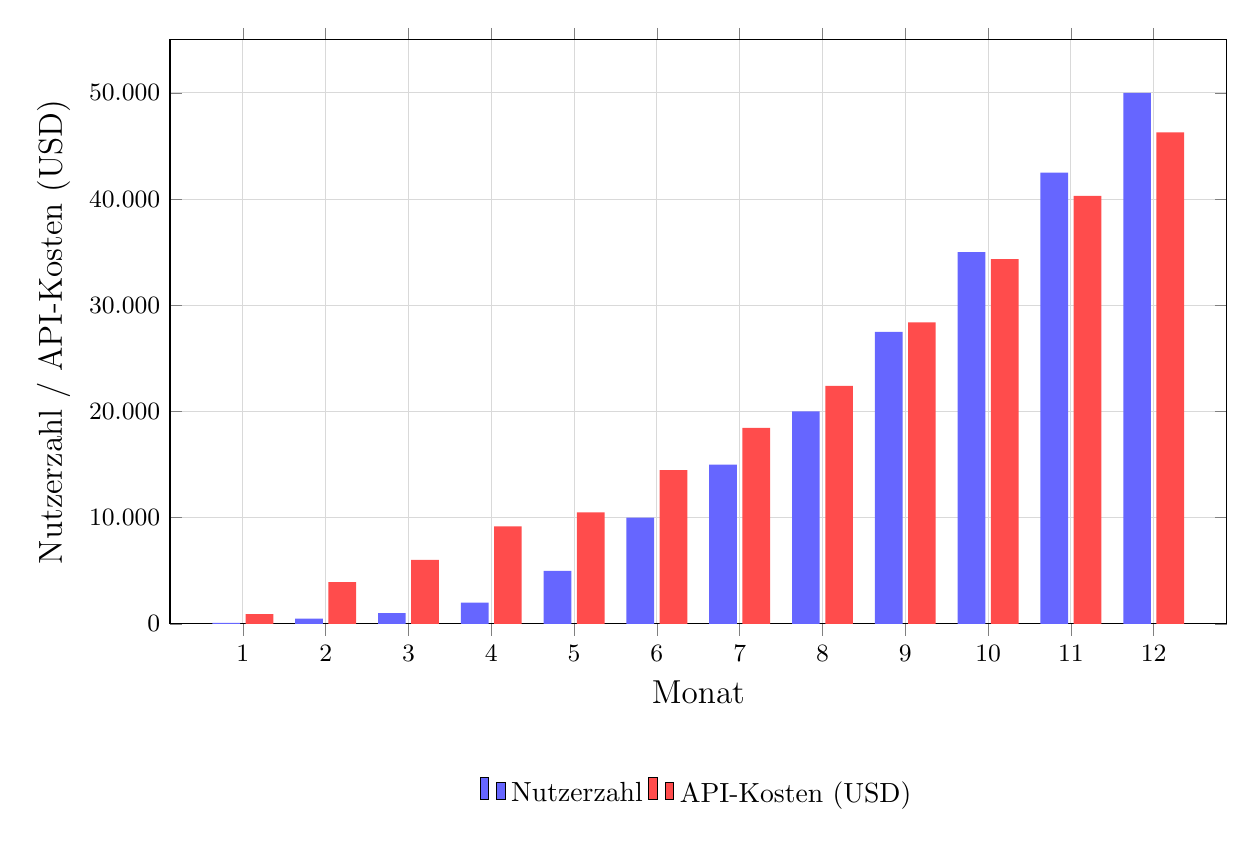
\begin{tikzpicture}
\begin{axis}[
    ybar,
    bar width=10pt,
    width=15cm,
    height=9cm,
    enlarge x limits=0.08,
    xlabel={Monat},
    ylabel={Nutzerzahl / API-Kosten (USD)},
    symbolic x coords={1,2,3,4,5,6,7,8,9,10,11,12},
    xtick=data,
    ymin=0,
    ymax=55000,
    % ---- WICHTIG: Kein 10^4 mehr ----
    scaled y ticks=false,
    yticklabel style={
        /pgf/number format/fixed,
        /pgf/number format/1000 sep={.}
    },
    % bessere Lesbarkeit
    tick label style={font=\small},
    label style={font=\large},
    grid=major,
    grid style={gray!30},
    % ---- Legende weiter nach unten ----
    legend style={
        at={(0.5,-0.25)},
        anchor=north,
        legend columns=2,
        draw=none
    },
]

% Nutzerzahl (blau)
\addplot[fill=blue!60, draw=none] coordinates {
(1,100) (2,500) (3,1000) (4,2000)
(5,5000) (6,10000) (7,15000) (8,20000)
(9,27500) (10,35000) (11,42500) (12,50000)
};

% API Kosten (rot)
\addplot[fill=red!70, draw=none] coordinates {
(1,910) (2,3920) (3,6020) (4,9170)
(5,10495) (6,14470) (7,18445) (8,22420)
(9,28382) (10,34345) (11,40307) (12,46270)
};

\legend{Nutzerzahl, API-Kosten (USD)}

\end{axis}
\end{tikzpicture}
\caption{Monatliche Nutzerzahlen und API-Kosten über 12 Monate}
\end{figure}

Wie aus der Abbildung ersichtlich ist, steigen sowohl die Nutzerzahl als auch die API-Kosten kontinuierlich an. Während die Nutzerzahl ein exponentielles Wachstum aufweist, wirken sich die gestaffelten Preisstrukturen der API zwar dämpfend auf die Kostensteigerung aus, dennoch ist eine frühzeitige Planung von Ressourcen und Budget unerlässlich. Die zugrunde liegende Preisstaffelung basiert auf dem nutzungsabhängigen Abrechnungsmodell der Google Maps Platform \cite{Google_Maps_Pricing2026}.

\subsection{Analyse der Server- und Hostingkosten in Abhängigkeit von den Nutzerzahlen}

Neben den variablen API-Kosten stellen auch Server- und Hostingkosten einen wesentlichen Bestandteil der operativen Ausgabenstruktur der Anwendung dar. Mit steigender Nutzerzahl erhöht sich die Systemauslastung hinsichtlich Rechenleistung, Speicherbedarf, Datenbankzugriffen sowie Netzwerktraffic. Insbesondere bei wachsender Anzahl gleichzeitiger Zugriffe (Concurrent Users) kann eine Skalierung der Serverinfrastruktur erforderlich werden, um Performance, Verfügbarkeit und Ausfallsicherheit sicherzustellen.

\begin{figure}[H]
\centering
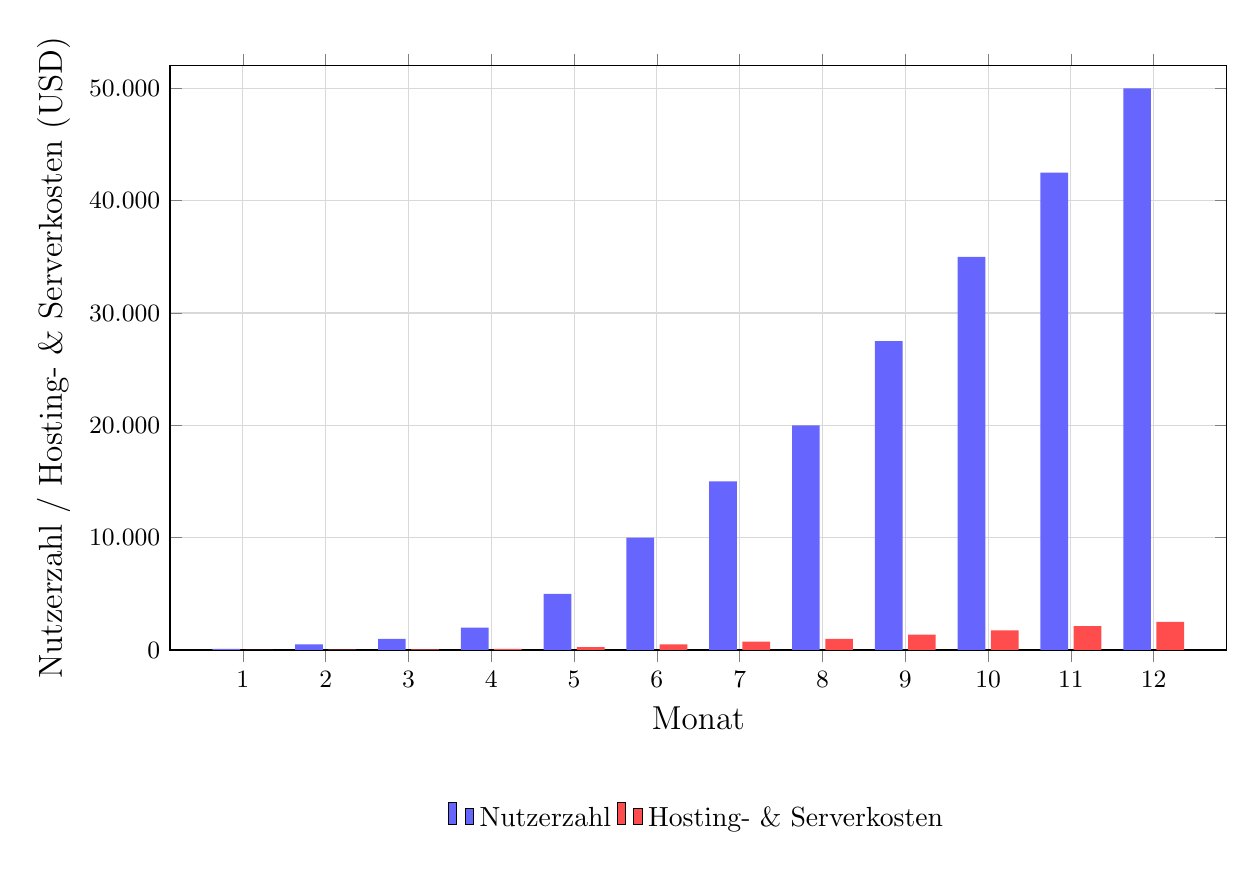
\begin{tikzpicture}
\begin{axis}[
    ybar,
    bar width=10pt,
    width=15cm,
    height=9cm,
    enlarge x limits=0.08,
    xlabel={Monat},
    ylabel={Nutzerzahl / Hosting- \& Serverkosten (USD)},
    symbolic x coords={1,2,3,4,5,6,7,8,9,10,11,12},
    xtick=data,
    ymin=0,
    ymax=52000,
    scaled y ticks=false,
    yticklabel style={
        /pgf/number format/fixed,
        /pgf/number format/1000 sep={.}
    },
    tick label style={font=\small},
    label style={font=\large},
    grid=major,
    grid style={gray!30},
    legend style={
        at={(0.5,-0.25)},
        anchor=north,
        legend columns=2,
        draw=none
    },
]

% Nutzerzahl (blau)
\addplot[fill=blue!60, draw=none] coordinates {
(1,100) (2,500) (3,1000) (4,2000)
(5,5000) (6,10000) (7,15000) (8,20000)
(9,27500) (10,35000) (11,42500) (12,50000)
};

% Hosting- & Serverkosten (rot) – 0,05 USD pro Nutzer
\addplot[fill=red!70, draw=none] coordinates {
(1,5) (2,25) (3,50) (4,100)
(5,250) (6,500) (7,750) (8,1000)
(9,1375) (10,1750) (11,2125) (12,2500)
};

\legend{Nutzerzahl, Hosting- \& Serverkosten}

\end{axis}
\end{tikzpicture}
\caption{Monatliche Nutzerzahlen und Hosting- \& Serverkosten über 12 Monate}
\end{figure}

Die Abbildung zeigt die monatliche Entwicklung der Nutzerzahlen (blaue Balken) sowie der daraus resultierenden Hosting- und Serverkosten (rote Balken) über ein Jahr.

Die Kosten wurden auf Basis realistischer Supabase-Infrastrukturpreise berechnet: Für jeden Nutzer fallen durchschnittlich etwa 0,05 USD pro Monat an, um Datenbank, Authentifizierung, Storage, API-Requests und Realtime-Funktionen bereitzustellen. Da die App WoSamma auf Supabase als BaaS setzt, übernimmt die Plattform sämtliche Backend-Dienste einschließlich Autoscaling, Load Balancing, Caching und Replikation. \cite{SupabaseBilling2026}

Mit zunehmender Nutzerzahl steigen die Gesamtkosten entsprechend, wobei durch die effiziente Skalierung der Supabase-Cloud der Preis pro Nutzer langfristig stabil bleibt oder tendenziell leicht sinkt. Dies verdeutlicht die wirtschaftliche und technische Skalierbarkeit, die durch die Nutzung eines modernen BaaS wie Supabase erreicht wird.

\subsection{Kumulierte Kosten in Abhängigkeit der Nutzerzahlen}

Die Abbildung zeigt die kumulierten Gesamtkosten (API + Hosting/Server) in Abhängigkeit der Nutzerzahlen über 12 Monate.  
Die Kosten steigen mit zunehmender Nutzerzahl, da zusätzliche Infrastruktur und API-Nutzung erforderlich sind.

\begin{figure}[H]
\centering
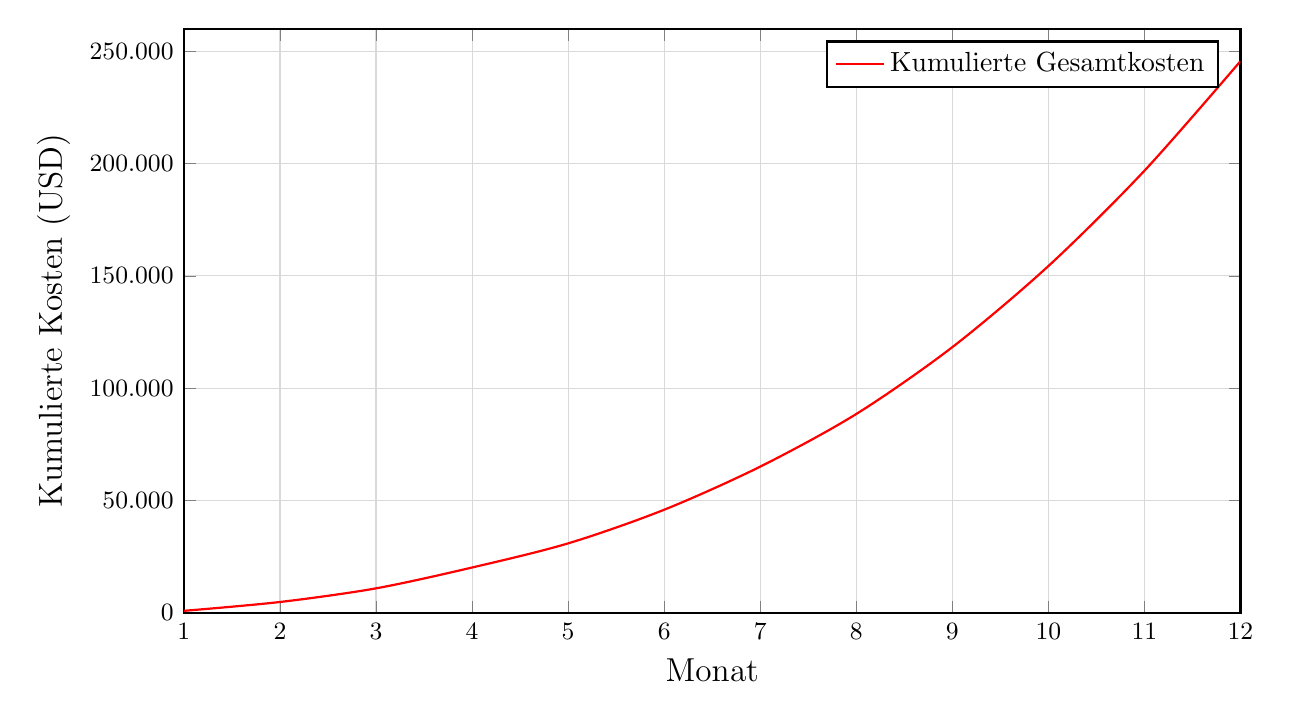
\begin{tikzpicture}
\begin{axis}[
    width=15cm,
    height=9cm,
    xlabel={Monat},
    ylabel={Kumulierte Kosten (USD)},
    xmin=1, xmax=12,
    ymin=0, ymax=260000,
    grid=major,
    grid style={gray!30},
    tick label style={font=\small},
    label style={font=\large},
    thick,
    scaled ticks=false,
    yticklabel style={
        /pgf/number format/fixed,
        /pgf/number format/1000 sep={.}
    },
    xtick={1,2,3,4,5,6,7,8,9,10,11,12},
    xticklabel style={font=\small},
]

% Neue kumulierte Kostenlinie
\addplot[smooth, thick, red] coordinates {
(1,915)
(2,4860)
(3,10930)
(4,20200)
(5,30945)
(6,45915)
(7,65110)
(8,88530)
(9,118287)
(10,154382)
(11,196814)
(12,245584)
};
\addlegendentry{Kumulierte Gesamtkosten}

\end{axis}
\end{tikzpicture}
\caption{Kumulierte Gesamtkosten über 12 Monate.}
\end{figure}

Die rote Kurve zeigt die kumulierten Gesamtkosten der App \textit{WoSamma} über 12 Monate. 
Dabei werden API-Kosten und Hosting über Supabase berücksichtigt. 
Die Nutzerzahlen steigen von 100 auf 50.000, die kumulierten Kosten ergeben sich aus der Summe der monatlichen Aufwendungen:

\[
\text{Kumulierte Kosten im Monat } n = \sum_{i=1}^{n} (\text{API-Kosten}_i + \text{Supabase-Kosten}_i)
\]

Die X-Achse zeigt die Monate, die Y-Achse die kumulierten Kosten in USD.

% ==================================================
\subsection{Einnahmen durch Werbung (Banner sowie Video-/Playable-Ads)}
Für die Werbeeinnahmen werden zwei Formate betrachtet: \textbf{Bannerwerbung} (als schmaler, dauerhaft eingeblendeter Balken in der App) sowie \textbf{Video-/Playable-Ads} als Hauptformat. Der Banner wird dabei \textbf{auf allen Seiten außerhalb des aktiven Spiels} angezeigt (z.\,B. Hauptmenü, Lobby, Profil, Einstellungen). \textbf{Im laufenden Spiel} wird kein Banner eingeblendet, um den Spielfluss nicht zu stören.
Die Berechnung erfolgt monatlich auf Basis der prognostizierten Nutzerzahlen.

\textbf{Basisannahmen:}
\begin{itemize}
    \item Monatliche aktive Nutzer entsprechen der Prognose.
    \item Anteil der Pro-Version-Nutzer: 2\% (somit 98\% Free-Nutzer sehen Werbung).
    \item 30 Tage pro Monat.
    \item \textbf{Video-/Playable-Ads:} durchschnittlich 3 Impressionen pro Free-Nutzer und Tag
    (abgeleitet aus Werbeplätzen nach Mehrspieler-Runden, Daily-Challenge und intervallbasiertem Einzelspieler).
    \item \textbf{Banner:} dauerhaft sichtbar \textit{außerhalb} des Spiels; Annahme: ein Free-Nutzer befindet sich im Mittel ca. 10 Minuten/Tag in Menüs/Lobbys,
    bei einem Refresh-Intervall von 60 Sekunden entspricht das \textbf{10 Banner-Impressionen pro Tag}.
    \item eCPM (theoretischer Mittelwert): Video/Playable = 25\,€/1000 Impr., Banner = 1{,}5\,€/1000 Impr.
\end{itemize}

\textbf{Formeln (pro Monat):}
\[
\text{Impr}_{video} = \text{FreeUser}\cdot 3 \cdot 30,\quad
\text{Umsatz}_{video} = \frac{\text{Impr}_{video}}{1000}\cdot 25
\]
\[
\text{Impr}_{banner} = \text{FreeUser}\cdot 10 \cdot 30,\quad
\text{Umsatz}_{banner} = \frac{\text{Impr}_{banner}}{1000}\cdot 1{,}5
\]

\begin{figure}[H]
\centering
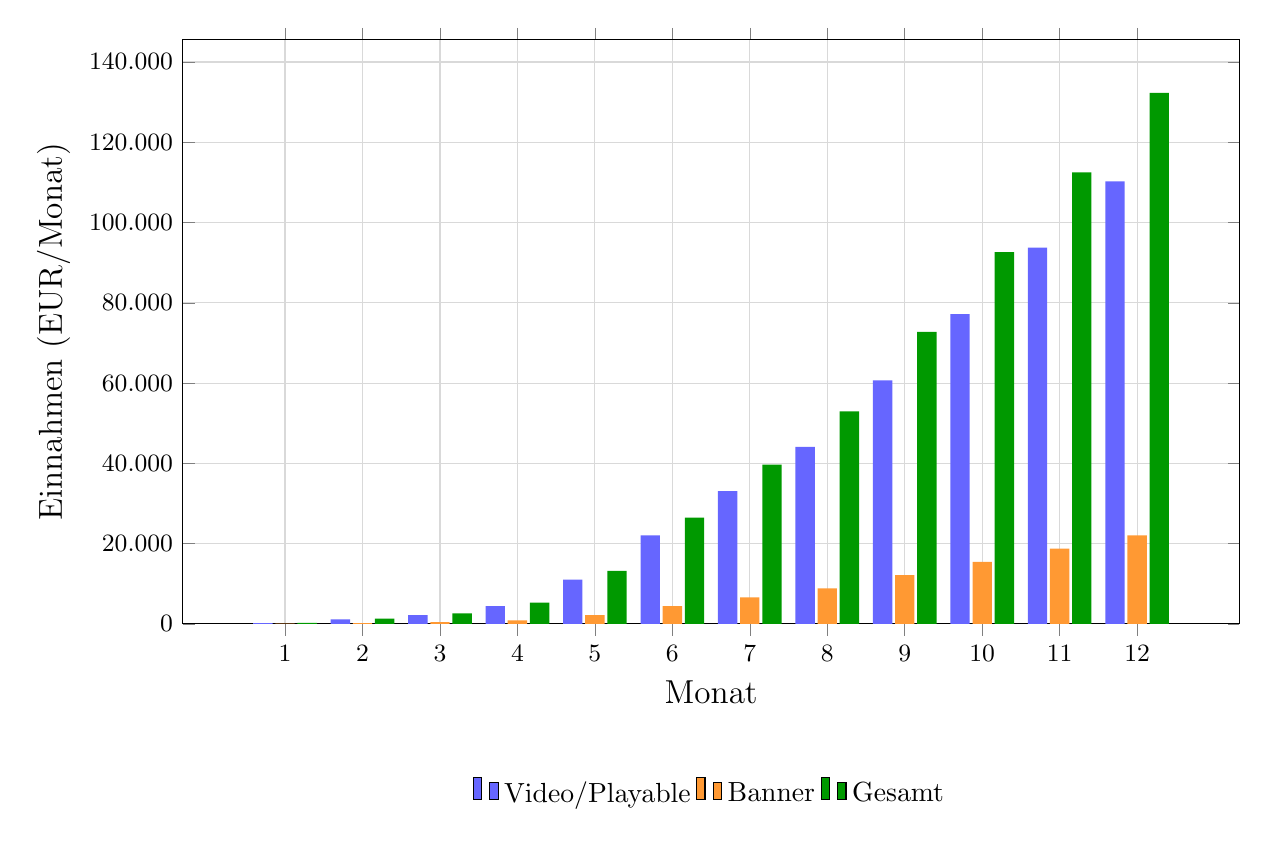
\begin{tikzpicture}
\begin{axis}[
    ybar,
    bar width=7pt,
    width=15cm,
    height=9cm,
    enlarge x limits=0.12,
    xlabel={Monat},
    ylabel={Einnahmen (EUR/Monat)},
    symbolic x coords={1,2,3,4,5,6,7,8,9,10,11,12},
    xtick=data,
    ymin=0,
    scaled y ticks=false,
    yticklabel style={
        /pgf/number format/fixed,
        /pgf/number format/1000 sep={.}
    },
    tick label style={font=\small},
    label style={font=\large},
    grid=major,
    grid style={gray!30},
    legend style={
        at={(0.5,-0.25)},
        anchor=north,
        legend columns=3,
        draw=none
    },
]

% Video Einnahmen
\addplot[fill=blue!60, draw=none, bar shift=-8pt] coordinates {
(1,220.50) (2,1102.50) (3,2205.00) (4,4410.00)
(5,11025.00) (6,22050.00) (7,33075.00) (8,44100.00)
(9,60652.50) (10,77205.00) (11,93757.50) (12,110250.00)
};

% Banner Einnahmen
\addplot[fill=orange!80, draw=none, bar shift=0pt] coordinates {
(1,44.10) (2,220.50) (3,441.00) (4,882.00)
(5,2205.00) (6,4410.00) (7,6615.00) (8,8820.00)
(9,12127.50) (10,15435.00) (11,18742.50) (12,22050.00)
};

% Gesamt Einnahmen
\addplot[fill=green!60!black, draw=none, bar shift=8pt] coordinates {
(1,264.60) (2,1323.00) (3,2646.00) (4,5292.00)
(5,13230.00) (6,26460.00) (7,39690.00) (8,52920.00)
(9,72780.00) (10,92640.00) (11,112500.00) (12,132300.00)
};

\legend{Video/Playable, Banner, Gesamt}

\end{axis}
\end{tikzpicture}
\caption{Monatliche Werbeeinnahmen getrennt nach Video-/Playable-Ads, Banner sowie Gesamterlös}
\end{figure}
% ==================================================
% ==================================================
\subsection{Einnahmen durch Pro-Abonnement (No-Ads)}
Das Pro-Abonnement wird als wiederkehrende Einnahmequelle bewertet, da laufende Betriebskosten (z.\,B. API-Nutzung) damit planbarer gedeckt werden können.
Für die folgende Modellrechnung wird die typische Abo-Quote angenommen.\cite{RevenueCat_Subscriptions2025}

\textbf{Basisannahmen:}
\begin{itemize}
    \item Anteil Pro-Nutzer: 2\% der monatlich aktiven Nutzer.
    \item Beispielhafter Preis: 4{,}99\,EUR pro Monat (\textit{finale Festlegung in der Kosten-Nutzen-Analyse je nachdem ob man die Kosten decken kann oder nicht}).
\end{itemize}

\textbf{Formel (pro Monat):}
\[
\text{Umsatz}_{Abo} = \text{User} \cdot 0{,}02 \cdot 4{,}99
\]

\begin{figure}[H]
\centering
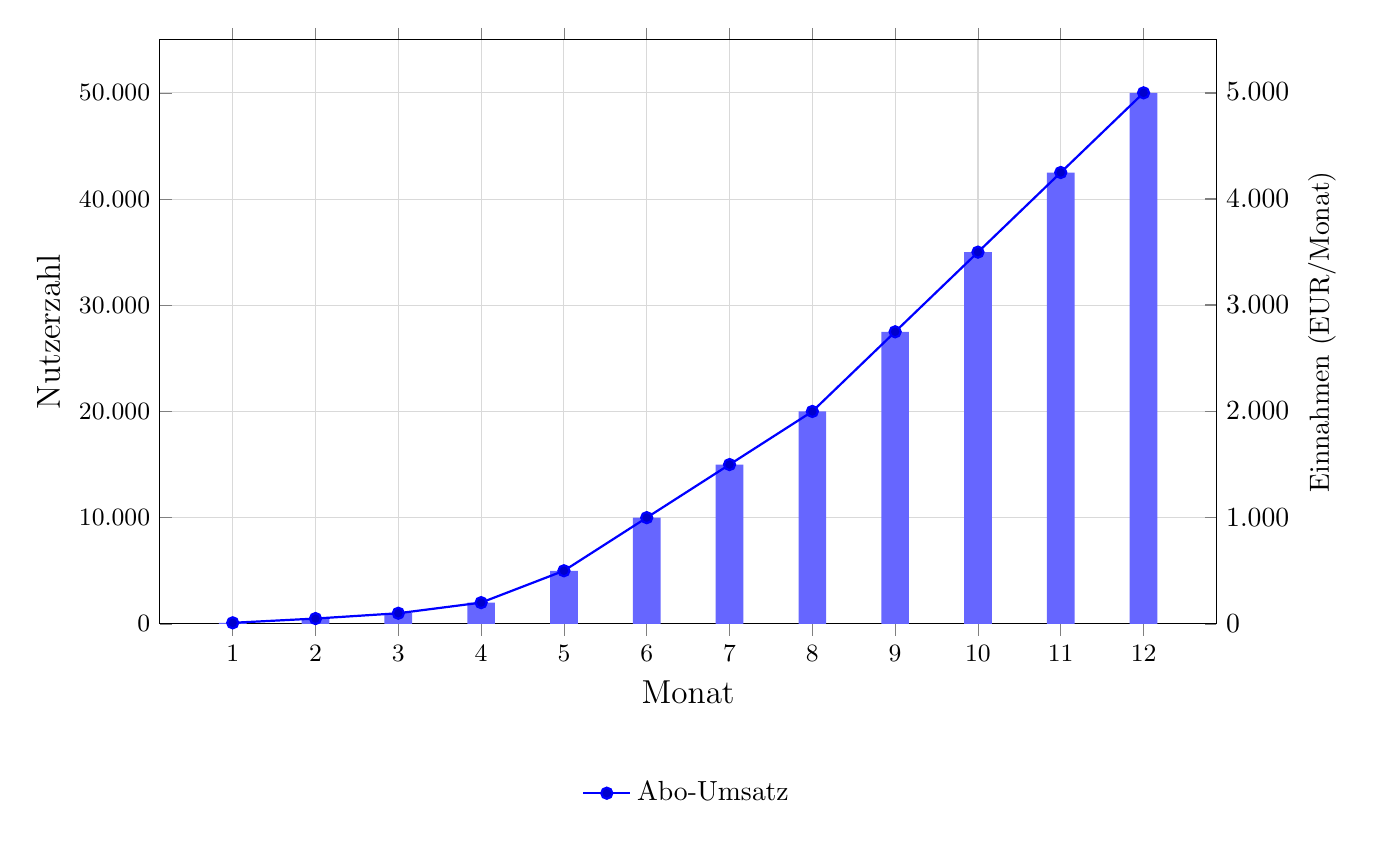
\begin{tikzpicture}
% --- Achse 1: Nutzer (Balken)
\begin{axis}[
    ybar,
    bar width=10pt,
    width=15cm,
    height=9cm,
    enlarge x limits=0.08,
    xlabel={Monat},
    ylabel={Nutzerzahl},
    symbolic x coords={1,2,3,4,5,6,7,8,9,10,11,12},
    xtick=data,
    ymin=0,
    ymax=55000,
    scaled y ticks=false,
    yticklabel style={
        /pgf/number format/fixed,
        /pgf/number format/1000 sep={.}
    },
    tick label style={font=\small},
    label style={font=\large},
    grid=major,
    grid style={gray!30},
]
\addplot[fill=blue!60, draw=none] coordinates {
(1,100) (2,500) (3,1000) (4,2000)
(5,5000) (6,10000) (7,15000) (8,20000)
(9,27500) (10,35000) (11,42500) (12,50000)
};
\end{axis}

% --- Achse 2: Einnahmen (Linie)
\begin{axis}[
    width=15cm,
    height=9cm,
    enlarge x limits=0.08,
    symbolic x coords={1,2,3,4,5,6,7,8,9,10,11,12},
    xtick=data,
    axis x line=none,
    axis y line*=right,
    ylabel={Einnahmen (EUR/Monat)},
    ymin=0,
    scaled y ticks=false,
    yticklabel style={
        /pgf/number format/fixed,
        /pgf/number format/1000 sep={.}
    },
    legend style={
        at={(0.5,-0.25)},
        anchor=north,
        legend columns=2,
        draw=none
    },
]
\addplot+[mark=*, thick] coordinates {
(1,9.98) (2,49.90) (3,99.80) (4,199.60)
(5,499.00) (6,998.00) (7,1497.00) (8,1996.00)
(9,2744.50) (10,3493.00) (11,4241.50) (12,4990.00)
};
\legend{Abo-Umsatz}
\end{axis}
\end{tikzpicture}
\caption{Monatliche Nutzerzahlen und theoretische Einnahmen durch das Pro-Abonnement}
\end{figure}
% ==================================================
% ==================================================
\subsection{Einnahmen durch In-App-Käufe (Profilbilder)}
In-App-Käufe werden als ergänzende Einnahmequelle betrachtet. In der App werden kosmetische Inhalte (Profilbilder) angeboten, die keinen spielerischen Vorteil erzeugen und daher als fair und UX-schonend gelten.

\textbf{Basisannahmen:}
\begin{itemize}
    \item Preis pro Profilbild: 0{,}99\,EUR.
    \item Kaufquote: 3\% der monatlich aktiven Nutzer kaufen im Monat ein Profilbild.
\end{itemize}

\textbf{Formel (pro Monat):}
\[
\text{Umsatz}_{IAK} = \text{User} \cdot 0{,}03 \cdot 0{,}99
\]

\begin{figure}[H]
\centering
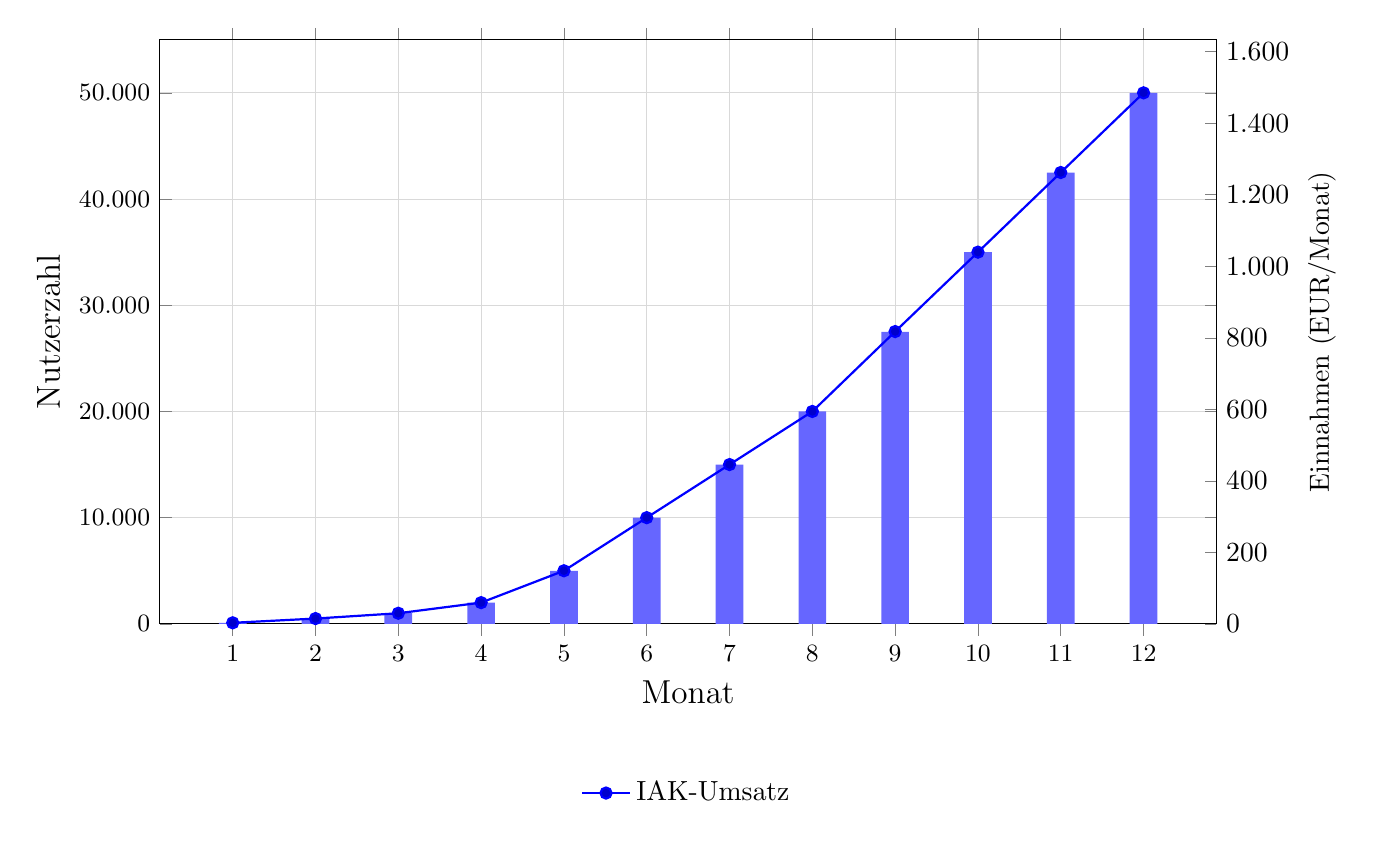
\begin{tikzpicture}
% --- Achse 1: Nutzer (Balken)
\begin{axis}[
    ybar,
    bar width=10pt,
    width=15cm,
    height=9cm,
    enlarge x limits=0.08,
    xlabel={Monat},
    ylabel={Nutzerzahl},
    symbolic x coords={1,2,3,4,5,6,7,8,9,10,11,12},
    xtick=data,
    ymin=0,
    ymax=55000,
    scaled y ticks=false,
    yticklabel style={
        /pgf/number format/fixed,
        /pgf/number format/1000 sep={.}
    },
    tick label style={font=\small},
    label style={font=\large},
    grid=major,
    grid style={gray!30},
]
\addplot[fill=blue!60, draw=none] coordinates {
(1,100) (2,500) (3,1000) (4,2000)
(5,5000) (6,10000) (7,15000) (8,20000)
(9,27500) (10,35000) (11,42500) (12,50000)
};
\end{axis}

% --- Achse 2: Einnahmen (Linie)
\begin{axis}[
    width=15cm,
    height=9cm,
    enlarge x limits=0.08,
    symbolic x coords={1,2,3,4,5,6,7,8,9,10,11,12},
    xtick=data,
    axis x line=none,
    axis y line*=right,
    ylabel={Einnahmen (EUR/Monat)},
    ymin=0,
    scaled y ticks=false,
    yticklabel style={
        /pgf/number format/fixed,
        /pgf/number format/1000 sep={.}
    },
    legend style={
        at={(0.5,-0.25)},
        anchor=north,
        legend columns=2,
        draw=none
    },
]
\addplot+[mark=*, thick] coordinates {
(1,2.97) (2,14.85) (3,29.70) (4,59.40)
(5,148.50) (6,297.00) (7,445.50) (8,594.00)
(9,817.43) (10,1039.50) (11,1262.25) (12,1485.00)
};
\legend{IAK-Umsatz}
\end{axis}
\end{tikzpicture}
\caption{Monatliche Nutzerzahlen und theoretische Einnahmen durch Profilbild-In-App-Käufe}
\end{figure}
% ==================================================
% ==================================================
\subsection{Kumulierte Gesamteinnahmen über 12 Monate}

Für die wirtschaftliche Gesamtbewertung der App ist neben den monatlichen Erlösen insbesondere die Entwicklung der \textbf{kumulierten Einnahmen} relevant. Dabei werden sämtliche Einnahmenquellen --- Werbung (Video-/Playable sowie Banner), Pro-Abonnement sowie In-App-Käufe --- fortlaufend aufsummiert. 

Die kumulierte Darstellung zeigt, wie sich die Gesamterlöse über das erste Betriebsjahr entwickeln und ermöglicht eine spätere Gegenüberstellung mit den kumulierten Kosten (z.\,B. API-, Hosting- oder Betriebskosten).

\begin{figure}[H]
\centering
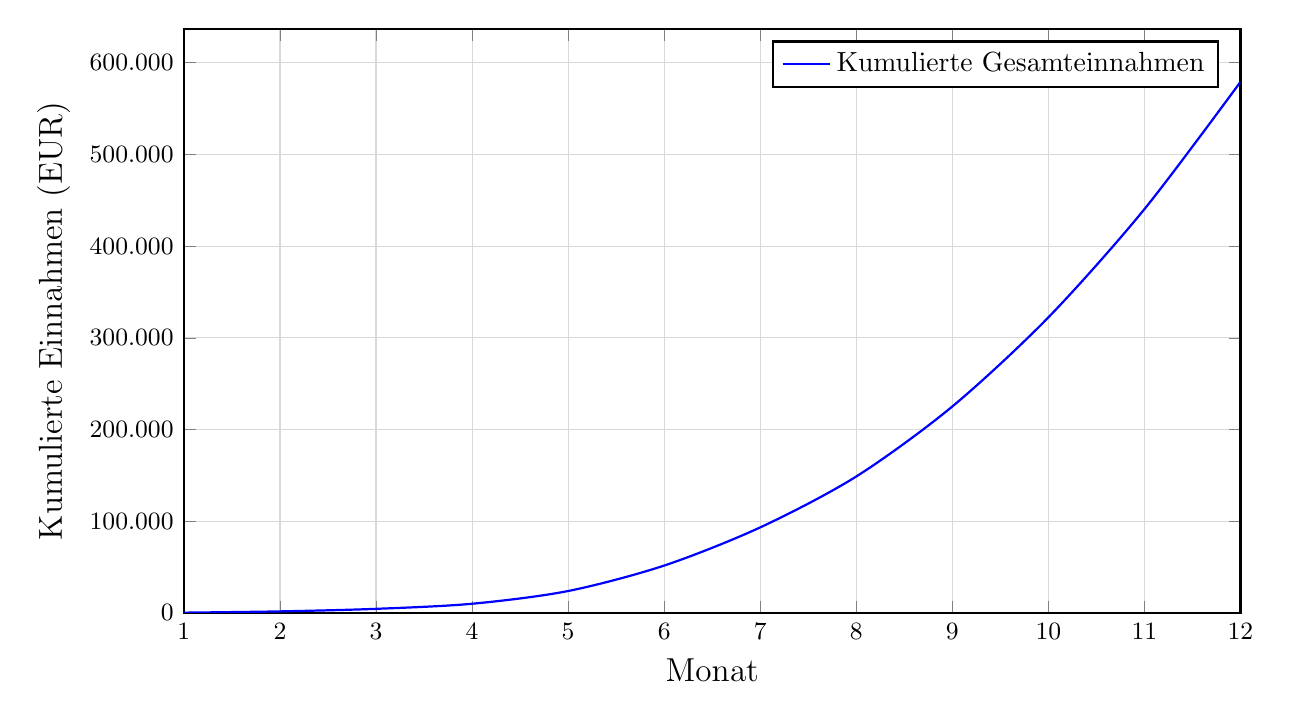
\begin{tikzpicture}
\begin{axis}[
    width=15cm,
    height=9cm,
    xlabel={Monat},
    ylabel={Kumulierte Einnahmen (EUR)},
    xmin=1, xmax=12,
    ymin=0,
    grid=major,
    grid style={gray!30},
    tick label style={font=\small},
    label style={font=\large},
    thick,
    scaled ticks=false,
    yticklabel style={
        /pgf/number format/fixed,
        /pgf/number format/1000 sep={.}
    },
    xtick={1,2,3,4,5,6,7,8,9,10,11,12},
    xticklabel style={font=\small},
]

\addplot[smooth, thick, blue] coordinates {
(1,277.55)
(2,1665.30)
(3,4440.80)
(4,9991.80)
(5,23869.30)
(6,51624.30)
(7,93256.80)
(8,148766.80)
(9,225108.73)
(10,322281.23)
(11,440284.98)
(12,579059.98)
};
\addlegendentry{Kumulierte Gesamteinnahmen}

\end{axis}
\end{tikzpicture}
\caption{Kumulierte Gesamteinnahmen aus Werbung, Pro-Abonnement und In-App-Käufen über 12 Monate}
\end{figure}
% ==================================================
% ==================================================
\subsection{Gegenüberstellung kumulierter Einnahmen und Kosten}

Zur abschließenden wirtschaftlichen Bewertung der App werden die kumulierten Gesamteinnahmen den kumulierten Gesamtkosten gegenübergestellt. 
Durch die fortlaufende Aufsummierung beider Werte über einen Zeitraum von zwölf Monaten lässt sich erkennen, ob und ab welchem Zeitpunkt die Einnahmen die Kosten decken und somit ein wirtschaftlicher Betrieb möglich ist.

Die folgende Grafik stellt die Entwicklung der kumulierten Einnahmen (aus Werbung, Pro-Abonnement und In-App-Käufen) sowie der kumulierten Kosten gemeinsam dar. 
Liegt die Einnahmenkurve über der Kostenkurve, wird ein Gewinn erzielt; liegt sie darunter, entstehen Verluste.

\begin{figure}[H]
\centering
\begin{tikzpicture}
\begin{axis}[
    width=15cm,
    height=9cm,
    xlabel={Monat},
    ylabel={EUR / USD (kumuliert)},
    xmin=1, xmax=12,
    ymin=0, ymax=600000,
    grid=major,
    grid style={gray!30},
    tick label style={font=\small},
    label style={font=\large},
    thick,
    scaled ticks=false,
    yticklabel style={
        /pgf/number format/fixed,
        /pgf/number format/1000 sep={.}
    },
    xtick={1,...,12},
    legend style={at={(0.5,-0.22)},anchor=north,legend columns=3,draw=none}
]

% Einnahmen
\addplot[name path=rev, smooth, thick, blue] coordinates {
(1,277.55)(2,1665.30)(3,4440.80)(4,9991.80)
(5,23869.30)(6,51624.30)(7,93256.80)(8,148766.80)
(9,225108.73)(10,322281.23)(11,440284.98)(12,579059.98)
};\addlegendentry{Kumulierte Einnahmen}


% Kosten
\addplot[name path=cost, smooth, thick, red] coordinates {
(1,915)(2,4860)(3,10930)(4,20200)(5,30945)(6,45915)
(7,65110)(8,88530)(9,118287)(10,154382)(11,196814)(12,245584)
};\addlegendentry{Kumulierte Kosten}


% Verlustbereich (rot)
\addplot[red!20,draw=none]
fill between[of=rev and cost,soft clip={domain=1:5.55}];
\addlegendentry{Verlust}

% Gewinnbereich (grün)
\addplot[green!25,draw=none]
fill between[of=rev and cost,soft clip={domain=5.55:12}];
\addlegendentry{Gewinn}
% Break-even Punkt
\addplot[only marks,mark=*,black] coordinates {(5.55,39220)};
\node[anchor=south,font=\small,fill=white]
at (axis cs:5.55,70000) {Break-even};

% Gewinntext am Ende
\node[anchor=north east,font=\small,fill=white]
at (axis cs:12,579059.98)
{Gesamtgewinn: 333.476};


\end{axis}
\end{tikzpicture}
\caption{Kumulierte Einnahmen und Kosten mit Gewinn- und Verlustbereich}
\end{figure}
Die Auswertung der kumulierten Einnahmen und Gesamtkosten über den betrachteten Zeitraum von zwölf Monaten zeigt deutlich, dass das Projekt wirtschaftlich tragfähig ist. Bereits nach wenigen Monaten wird der Break-even-Punkt erreicht, ab dem die Einnahmen die anfallenden Kosten übersteigen und ein kontinuierlicher Gewinn erzielt wird. Gegen Ende des ersten Jahres ergibt sich ein klar positiver Gesamtgewinn, wodurch die Rentabilität des Geschäftsmodells bestätigt wird.

Bei den durchgeführten Berechnungen wurde zudem nicht berücksichtigt, dass für Einnahmen aus Abonnements und In-App-Käufen Provisionen an die jeweiligen App-Stores abgeführt werden müssen. Dieser Abzug würde die tatsächlichen Nettoerlöse zwar geringfügig reduzieren, hätte jedoch keinen wesentlichen Einfluss auf das Gesamtergebnis, da die Einnahmen aus Werbung im Vergleich zu Abonnements und In-App-Käufen den deutlich größten Anteil darstellen. Der verbleibende Abzug würde somit nur einen relativ kleinen Teil der Gesamteinnahmen betreffen:\\
Für die wirtschaftliche Gesamtbetrachtung werden die Einnahmen aus Pro-Abonnement und In-App-Käufen über den gesamten Zeitraum von 12 Monaten kumuliert.

Die aufsummierten Einnahmen betragen:
\begin{itemize}
    \item Pro-Abonnements gesamt: 20\,818{,}28\,EUR
    \item In-App-Käufe gesamt: 6\,196{,}10\,EUR
\end{itemize}

Damit ergeben sich kombinierte Einnahmen von:
\[
20\,818{,}28 + 6\,196{,}10 = 27\,014{,}38\,\text{EUR}
\]

Auf diese Umsätze fällt eine Store-Provision von etwa 15\,\% an:
\[
27\,014{,}38 \times 0{,}15 \approx 4\,052{,}16\,\text{EUR}
\]

Nach Abzug der Store-Provision verbleiben somit:
\[
27\,014{,}38 - 4\,052{,}16 \approx 22\,962{,}22\,\text{EUR}
\]
Insgesamt zeigt die wirtschaftliche Betrachtung, dass das Projekt mit einem deutlichen Gesamtgewinn(333.476 USD, mit Abzug von App-Store-Gebühren: 329.423 USD) abschließt und somit als klarer Erfolg bewertet werden kann, da sämtliche Kosten gedeckt sind und darüber hinaus ein nachhaltiger finanzieller Überschuss erzielt wird.